\setcounter{tocdepth}{5}

\section{Tervezés}

\subsection{Bevezető}

Ebben a részben elsőként leírom, illetve összehasonlítom a multimédia üzenetküldő rendszer megvalósítási lehetőségeit, majd az általam kiválasztott módszer funkcionális egységeit,  részletesen tárgyalva azok szerepét és egymással való kapcsolatát.

\subsection{A megvalósítási lehetőségek}

Nézzük meg, hogy az IMS használata esetén milyen lehetőségek kínálkoznak a csoportos üzenetküldés megvalósítására. A megoldási lehetőségek ismertetése során kitérek azok előnyeire, hátrányaira, illetve a felmerülő problémákra.

\subsubsection{SIP MESSAGE üzenetek használata}
\label{sec:sip_message}

Első megoldásként kézenfekvőnek tűnhet, hogy a SIP protokoll által nyújtott MESSAGE típusú üzenet törzsében küldjük el a multimédia üzenetet a címzetteknek. Ennek a megoldásnak az az előnye, hogy nem kell másik protokollt használni az üzenetek átviteléért, hanem a SIP protokoll nyújtotta funkciókat alkalmazzuk. A megoldás előnye viszont eltörpül a hátrányok mellett. Először is a MESSAGE típusú üzenetnek nem adható meg egynél több címzett, így minden címzettnek különálló MESSAGE üzenetben kellene elküldeni ugyanazt a tartalmat. Ez a megszorítás redundanciához vezet, mivel a feladónak ugyanazt az üzenetet minden címzettnek külön-külön el kell küldenie, ami a válaszidőt is jelentősen megnöveli. Erre a problémára megoldást jelenthet, ha az üzenetet egy alkalmazás szerveren keresztül küldjük, ahol a szerver feladata az üzenet továbbítása az a címzetteknek. Ebben az esetben a feladó és a szerver között csak egyszer kerülne átküldésre az üzenet, ami a szűkebb sávszélességű felhasználói hálózatok esetén hatalmas előnyt jelent a többszörös küldéshez képest. Ahhoz, hogy ez a megvalósítás működhessen, a felhasználókból csoportokat kell létrehozni, és a MESSAGE üzenetet a címzettek URI-ja (Uniform Resource Identifier) helyett a csoport URI-jával címezni. Amikor az alkalmazás szerver megkapja ezt az üzenetet, a csoport azonosító alapján valamilyen módon -- pl. saját adatbázisból -- megkeresi azokat a felhasználókat, akik tagjai a csoportnak, és mindegyik csoporttagnak egyesével elküldi a kapott üzenet másolatát. Ebben az esetben szükség van az alkalmazás szerver oldalán egy olyan funkcióra, ami a csoportkezelést megvalósítja.
További problémát jelent, ha a küldött multimédia mérete meghaladja a MESSAGE üzenet törzsébe maximálisan megadható 1300 oktetet\footnote{RFC 3428 - Session Initiation Protocol Extension for Instant Messaging \cite{rfc3428}}. Ilyenkor a tartalmat a küldő oldalon kisebb darabokra kell tördelni, a darabokat külön üzenetekben elküldeni, majd a vevő oldalon a kisebb részekből a teljes üzenetet rekonstruálni. A probléma gyökere, hogy a SIP MESSAGE üzenettípus nem támogatja egy üzenet több darabban való átvitelét. A MESSAGE üzenet fejlécében nincs lehetőség olyan paramétert megadni, amiből a vevő egyértelműen el tudja dönteni, hogy a beérkező MESSAGE üzenetek közül melyik hordozza ugyanazon tartalom egy-egy darabját, és melyik nem, amiből következően rekonstruálni sem tudja azt. További gond, hogy az üzenetek nem sorszámozottak, így az eredeti küldési sorrendet sem tudnánk visszaállítani. Ezek a problémák abból fakadnak, hogy a MESSAGE üzenet használatát elsősorban rövid szöveges üzenetek továbbítására találták ki, és nem nagy multimédia tartalmakhoz. 
A megoldás hátrányainak sorát bővíti az is, hogy nem támogatott a késleltetett üzenetküldést sem. Utóbbi problémát -- hasonlóan a többszörös küldéshez -- orvosolhatnánk az alkalmazás szerver használatával, amely eltárolná azokat az üzeneteket, amelyek a nem elérhető címzetteknek mennek, és a szerver akkor kézbesítené azt, amikor a címzett elérhetővé válik.

{\color{red}(IDE MÉG RFC3428-ból PÁR DOLOG)
(Leírni még, hogy a vevők válasza többször jön, stb...)}

\subsubsection{Több címzettel rendelkező üzenetek használata}
\label{sec:mr_message}

Mint ahogy \aref{sec:sip_message}.~fejezetben láthattuk, a SIP specifikáció nem nyújt hatékony megoldást a több címzettű üzenetek továbbítására. Ebben az alpontban leírt megoldás abban tér el az előzőhöz képest, hogy az üzenet fejlécben lehetőség van több címzettet megadni. A folytatásban az ilyen típusú üzenetet több címzettel rendelkező, azaz MR (Multi Recipient) üzenetnek fogom nevezni. A több címzett megadásának a lehetősége jelentős előnyt jelent az alap SIP MESSAGE-et használó megoldáshoz képest. Először is, a feladónak elég csak egyszer elküldeni az üzenetet a CSCF felé, és nem annyiszor, ahány címzettje van az üzenetnek. Ez jelentősen lecsökkenti a hálózati erőforrások használatát. Másodszor, mivel a címzettek az MR üzenet fejlécében helyezkednek el, így az erre alkalmas hálózati szerverek a fejléc adatokat felhasználva képesek az üzeneteket hatékonyan eljuttatni az összes címzettnek anélkül, hogy az üzenet törzsét meg kellene vizsgálniuk. Tegyük fel, hogy a feladó hálózatában lévő S-CSCF, miután megkapja feladótól az MR üzenetet, annak minden címzettjére meghatározza az adott címzett felé vezető következő állomást (next hop CSCF), ahová továbbítani kell azt. Abban az esetben, ha kettő vagy több címzett esetén ugyanaz a next hop, akkor az S-CSCF abba az irányba MR üzenetként küldi tovább az üzenetet. Ha minden címzett next hop CSCF-je különbözik egymástól, akkor a szerver az egyes next hop-oknak hagyományos üzenetben küldi el annak egy-egy másolatát. Mivel a hálózatban található összes CSCF hasonlóan viselkedik, mint a feladót kiszolgáló S-CSCF, ezzel a módszerrel két szerver között ugyanaz az üzenet pontosan egyszer kerül átvitelre. Az üzenet terjedésének folyamatát \aref{fig:mrflow}.~ábrán követhetjük nyomon. Jól látható, hogy ezzel a módszerrel minden linken kizárólag egyszer küldjük át ugyanazt az üzenetet, ellentétben az aktuális IMS javaslattal, miszerint több címzett esetén egy linken többször kellene átküldeni ugyanazt az üzenetet (Például a III-as, IV-es és V-ös linken). Abban az esetben, ha egy olyan CSCF vesz egy MR üzenetet, amely nem képes MR üzeneteket kezelni, akkor a küldő CSCF felé hibaüzenetet küld. Ilyenkor a küldő CSCF újra elküldi az üzenetet hagyományos SIP üzenetként, minden címzettre külön-külön. 

\begin{figure}[htbp]
\center
\resizebox{10cm}{!}{
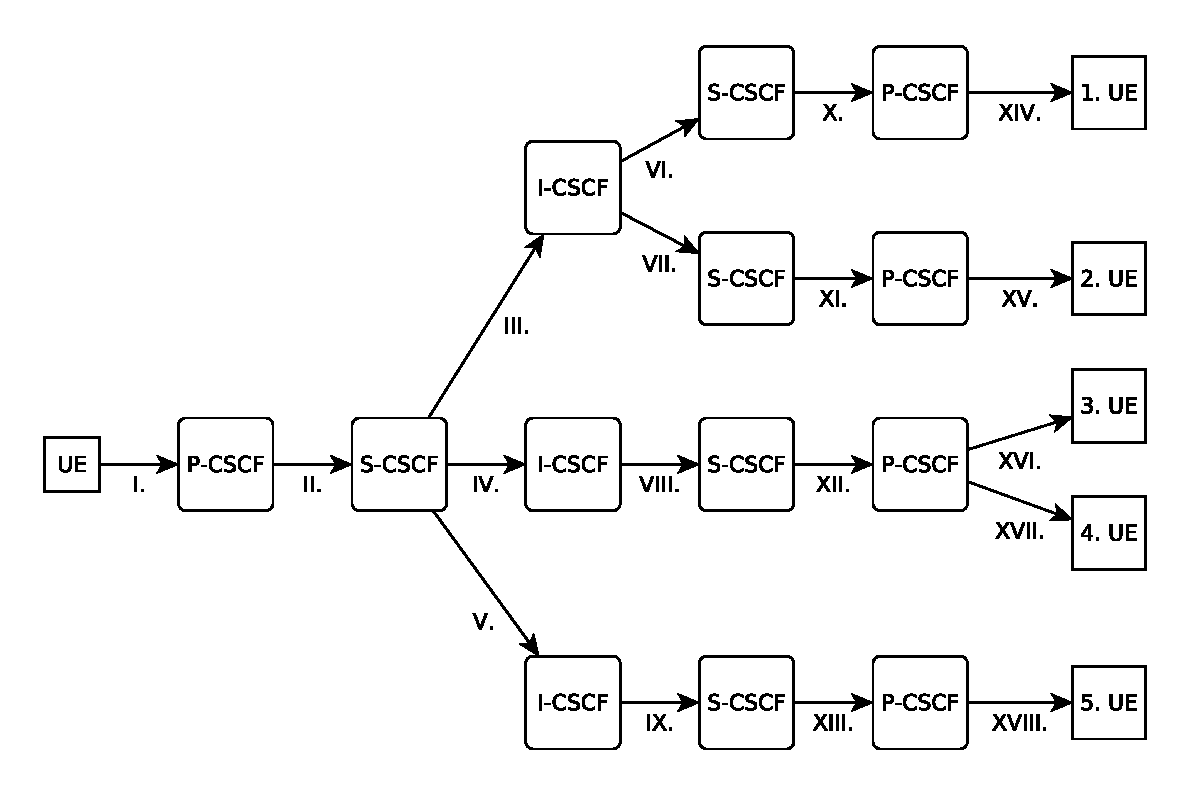
\includegraphics{img/MR-flow.eps}}
\caption{Az MR üzenetküldés folyamata}
\label{fig:mrflow}
\end{figure}

Mivel egy multimédia üzenet viszonylag nagy méretű is lehet, nagy valószínűséggel nem fér bele egyetlen MR üzenet törzsébe. Utóbbi probléma abból ered, hogy az IP hálózatokban maximalizálva van a hálózatba küldhető csomag mérete (MTU - Maximum Transmission Unit\footnote{IPV4-nél ez mekkora? Minimum 576 byte}). Hasonlóan a SIP MESSAGE üzeneteket használó megoldáshoz, itt is darabolni kellene a multimédia üzenetet több kisebb csomagra. Mivel az MR csomagok akár különböző útvonalon is eljuthatnak a címzettnek, a vételi oldalon való a csomagok eredeti sorrendjének visszaállíthatónak kell lennie. Amennyiben az MR üzenet fejlécében lehetőség lenne elhelyezni olyan mezőket, amelyek a helyes sorrend visszaállítását szolgálják, akkor a megoldás jelentősen jobb lenne, mint a SIP MESSAGE-et használó megvalósítás. Itt is általános feladatként jelentkezik a késleltett üzenetkézbesítés problémája, ami egy köztes alkalmazás szerver használatával megvalósítható lenne.

A vételi oldalon a kliensek, miután megkapták az MR kéréseket, nyugtázzák azokat. A cél itt is az, hogy a nyugták küldéséből eredő, a feladó és az őt kiszolgáló S-CSCF közötti linken folyó üzenetforgalmat minél jobban lecsökkentsük anélkül, hogy az IMS komponensek viselkedését alapvetően megváltoztatnánk. Ha a feladót kiszolgáló S-CSCF nem kompatibilis az MR üzenetekkel, akkor minden egyes nyugtát a hagyományos módon, egyesével továbbít a feladónak. Abban az esetben viszont, amikor az említett S-CSCF képes kezelni az MR üzeneteket, a hozzá beérkező, azonos típusú nyugtákra -- pl. 200 OK -- adott időtartamig vár, majd a nyugtákból összeállít egy MR választ, és csak ezt küldi el a feladónak, amivel jelentősen csökkenti a kérdéses link forgalmát.

\subsubsection{Üzenet továbbítása RTP protokoll segítségével -- {\color{red}IDE LEHET A VXML-es MRF-es megoldást kellene írni}}

{\color{red}Ezzel az a baj, hogy a video formátum erősen limitált. csak 3gp. Nem tudom, hogyan lehet képet átvinni. Ez főleg az interakciók miatt jó. max átvitt hang hossz is asszem limitált. Nem tudom, hogy erről kellene-e egyáltalán írni.}


\subsubsection{Üzenet továbbítása MSRP protokollal}
\label{sec:msrp_message}

Ez a megoldási javaslat a multimédia üzenetek felhasználók közötti átvitelére az MSRP (Message Session Relay Protocol) protokollt használja. Az MSRP -- a SIP-hez vagy a HTTP-hez hasonlóan -- egy szöveges, alkalmazás rétegbeli protokoll. A protokoll kapcsolat orientált adatátvitelt (session mode) tesz lehetővé, aminek számos előnye van a különálló, független üzenetcsomagok küldéséhez képest (paging mode).
Ezen előnyök közé tartozik, hogy a kommunikációs felek explicit felépítenek egymás között egy kommunikációs csatornát az üzenet csomagok átvitelére. A kapcsolat léte magában foglalja az összefüggő üzenet csomagok biztonságos, sorrendhelyes átvitelét, valamint a garantált kézbesítést is. Minden MSRP üzenet vagy egy kérés, vagy egy válasz. Az üzenetek fejlécből és törzsből állnak. A fejlécben az MSRP kapcsolatot, illetve a törzsben lévő -- szöveges vagy bináris -- tartalmat leíró információk találhatóak. Az MSRP kapcsolat felépítése SIP és SDP (Session Description Protocol) protokoll~\cite{rfc4566} segítségével történik. Az MSRP csomagok felépítésének leírása \aref{sec:msrp_chunks}.~fejezetben található. A protokollról részletesebben az~\cite{rfc4975} irodalomban olvashat. Az SDP protokoll egy olyan szabályegyüttes, amely a multimédiás tartalmakat továbbító kapcsolatok paramétereit írja le. Ilyen paraméter többek között a kapcsolat sávszélessége, a kapcsolaton átvitelre kerülő multimédiát leíró információk, az átviteli protokoll, a kommunikációs IP cím és port, stb. A kapcsolatot felépítő kommunikációs felek az SDP protokoll alapján leírják a rájuk jellemző paramétereket, majd SIP protokoll segítségével ,,megbeszélik'' egymással a felépíteni kívánt kapcsolatokat, azaz megoszják egymás között az SDP protokollal megadott paramétereket. 

Mivel a címzettek csoportjában lehet olyan felhasználó, aki az üzenet küldésének pillanatában nem elérhető, így a késletetett kézbesítés problémája ebben az esetben is felmerül. Utóbbi problémára itt is megoldást nyújt az, ha a kliensek közé egy alkalmazás szervert helyezünk el, amely többek között a késletetett üzenet kézbesítését is végzi. A köztes szerver használata a hálózati forgalmat is csökkenti, mivel a feladó és a szerver közötti, jellemzően alacsony sávszélességű (pl. rádiós) linken csak egyszer kerül átvitelre a -- gyakran nagy méretű -- multimédia üzenetet, szemben azzal az esettel, amikor a feladó minden címzettre külön-külön elküldi azt. Miután sikeresen átvitelre került a multimédia üzenet, a feladónak a címzettek listáját valamilyen módon, például egy SIP MESSAGE üzenet törzsében kézbesíteni kell a szerver felé. Mivel ez a lista jellemzően rövid szöveges üzenet, így belefér egyetlen SIP MESSAGE üzenetbe. A megoldás hátránya az MSRP kapcsolat felépítésének költsége, ami viszont a kapcsolat tényéből fakadó, már fentebb említett előnyökhöz képest elhanyagolható.

{\color{red} (... üzenet kézbesítés, előny, hátrány)}
\\
A dolgozatban a szolgáltatás fejlesztése során a fentebb leírt megoldások közül a legutolsó, MSRP protokollt használó megoldás használata mellett döntöttem. A SIP MESSAGE üzenetek használata nem célszerű \aref{sec:sip_message}.~fejezetben leírt számos hátránya miatt. \Aref{sec:mr_message}.~fejezetben tárgyalt MR üzenetet használó csoportos üzenetküldési megoldás jelenleg csak ajánlás formájában létezik, bárminemű szabványosítási eljárás jelenleg nincs folyamatban a témával kapcsolatban. Az MSRP protokollal való megvalósítás előnye a többi megoldási javaslattal szemben, hogy -- az IMS-ben jelen lévő --szabványosított eszközök használatára épít, illetve az adatátvitel kapcsolatorientált jellege következtében megbízható üzenetküldés valósítható meg. 

\subsection{Funkcionális terv}

A rendszer alapvetően a klasszikus kliens-szerver architektúrát valósítja meg. A kliensek azok, akik létrehozzák a multimédia üzeneteket, majd a szerver köz\-ve\-tí\-té\-sé\-vel elküldik azt más kliensek egy meghatározott csoportjának. A szerver adatbázisban tárolja a multimédia üzenethez tartozó adatokat, mint például a feladó neve, SIP azonosítója, a címzettek nevei, a multimédia tartalom, stb. A küldő kliens az átvitel si\-ke\-res\-sé\-gé\-ről folyamatos értesítést kap a szervertől. A szerver, miután sikeresen megkapta az új üzenetet, az online címzetteknek -- egy SIP MESSAGE üzenet törzsében -- azonnal értesítést küld erről. Az említett üzenet törzsének részletes ismertetése a \aref{sec:sip_message} fejezetben található. Egy kliens, amikor az új üzenetről értesítést kap a szervertől, a tényleges multimédia üzenetről kapott leíró információk alapján eldöntheti, hogy érdekli-e őt az üzenet, vagy sem. Ilyen leíró információ az üzenet feladójának adatai, az üzenet tárgya, valamint az üzenet tartalmának típusa, úgy mint kép, hang vagy videó, illetve a küldés dátuma. A kapott információk alapján a címzett eldöntheti, hogy érdekli őt az üzenet tényleges multimédia tartalma vagy sem, és ezáltal a döntésnek megfelelő akciót végrehajtsa (azaz megtekintse a multimédia üzenetet vagy sem). 

A rendszer magasszintű modelljét \aref{fig:model}.~ábra szemlélteti.

\begin{figure}[htbp]
\center
\resizebox{12.5cm}{!}{
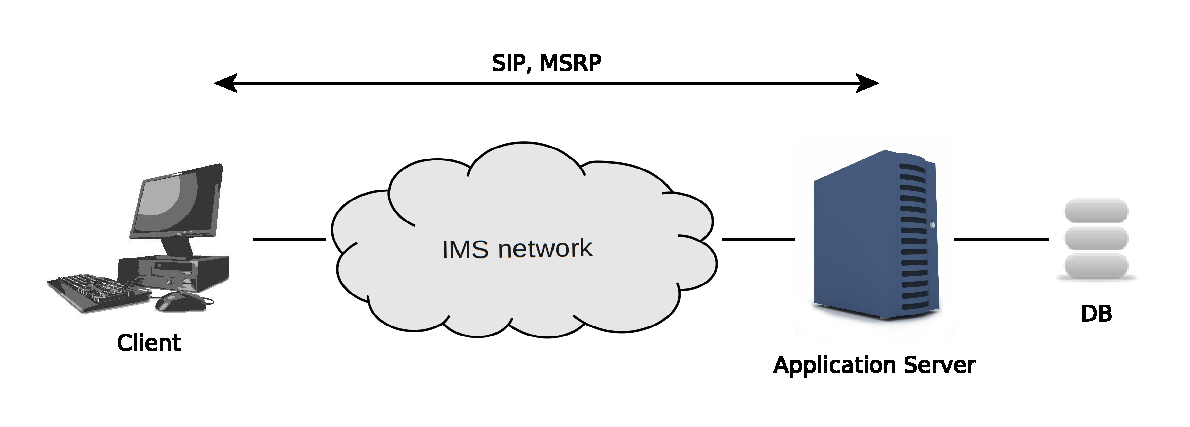
\includegraphics{img/system_MSRP_black_2.eps}}
\caption{A rendszer magasszintű modellje}
\label{fig:model}
\end{figure}

A rendszer az alábbi részekből épül fel:
\begin{mydescription}
\item[Kliens PC:] A felhasználó ezen keresztül éri el a szolgáltatást.
\item[Alkalmazás szerver:] Az üzenet fogadását és a címzetteknek való kézbesítést valósítja meg.
\item[Adatbázis szerver:] Az üzenethez tartozó adatok tényleges tárolását végzi.
\end{mydescription}

A következő fejezetekben az egyes elemek funkciójának részletes tárgyalása következik.

\subsubsection{Kliens}
\label{sec:kliens_pc}

A felhasználó ezen keresztül éri el az IMS hálózatot, azaz magát az üzenetküldő szolgáltatást is, ebből fakadóan a PC eszköznek rendelkeznie kell hálózati kapcsolattal. Miután a kliens oldali üzenetküldő szolgáltatást használó alkalmazás elindult, a felhasználó SIP URI-ját tartalmazó üzenetet periodikusan elküld a szerver oldalnak. Ez a periodikus ,,regisztráció'' azért szükséges, hogy a szerver oldal tisztában legyen azzal, hogy pillanatnyilag melyik felhasználó érhető el. A szerver amikor új multimédia üzenetet kap egy felhasználótól, értesíteni tudja a címzettek közül azokat, akik aktuálisan elérhető állapotban vannak. Az alkalmazás bezárásakor a kliens oldal ,,leiratkozó'' értesítést küld a szerver felé arról, hogy innentől kezdve a szóban forgó kliens nem elérhető. A regisztrációs üzenet küldésének periodikus jellege azért fontos, mert a kliens alkalmazás bármilyen hibás leállása esetén nem garantált az említett leiratkozó üzenet továbbítása a szerver felé. Utóbbi esetben az adott felhasználó elérhető kliensek listájáról való törlését a periódusidő lejárta után autómatikusan elvégzi a szerver oldal.

A felhasználó multimédia üzenetet küldhet más, általa ismert felhasználók csoportjának. Az elküldendő multimédia üzenet többféleképpen állhat a kliens rendelkezésére. Egyik lehetséges opció, hogy az elküldenő üzenethez tartozó multimédia tartalom fájlrendszeren már a felhasználó rendelkezésére áll kép, hang vagy videó fájl formájában. Ebben az esetben a küldő kliens fájlrendszeren való tallózással választhatja ki a multimédia tartalmat. A tartalom létrehozásának egy másik lehetséges módja, hogy a felhasználó a számítógépéhez kapcsolódó audiovizuális eszközökkel (mikrofon és kamera) maga készíti el a multimédia üzenethez multimédia felvételt. Miután az elküldendő multimédia üzenethez a tartalom a felhasználó rendelkezésére áll, valamilyen módon el kell küldeni a szerver oldalnak. A tartalom kliens-szerver közötti átvitele MSRP protokoll szerint történik.

{\color{red}Ezeket inkább a megvalósítási tervbe kellene tenni. Vagy nem?}

Az üzenetküldés folyamatát \aref{fig:sending_proc}.~ábrán láthatjuk. A folyamat első lépéseként a küldő kliens és a szerver között fel kell építeni egy MSRP kapcsolatot, amelyen keresztül a multimédia üzenet átvitele történik. Egy MSRP kapcsolat minden esetben egy kliens és a szerver között épül fel, két kliens közvetlenül egymáshoz soha nem csatlakozik. Amikor az MSRP kapcsolat sikeresen felépült, a feladó ezen kapcsolaton keresztül MSRP csomagok\footnote{Az MSRP csomag felépítése \aref{sec:msrp_chunks}.~fejezetben található} formájában továbbítja a multimédia üzenetet a szervernek. A szerver minden MSRP csomag vételét nyugtázza a küldő kliens felé. Miután a teljes üzenet sikeresen megérkezett a szerver oldalra, a a kliens bontja az MSRP kapcsolatot. A folyamat utolsó lépéseként a felhasználó egy SIP MESSAGE típusú üzenet törzsében elküldi a szervernek a címzettek listáját, illetve opcionálisan egyéb, az elküldött multimédia üzenetre jellemző információt. A címzett lista, illetve a kiegészítő információk XML (Extensible Markup Language) formátumban kerülnek átvitelre. Mivel az említett XML rövid, így az belefér egyetlen SIP MESSAGE üzenetbe. Miután a szerver sikeresen megkapta az XML-t tartalmazó üzenetet, a multimédia tartalommal együtt adatbázisban eltárolja azt, majd nyugtázza a sikeres vételt a feladó felé.

\begin{figure}[htbp]
\center
\resizebox{10cm}{!}{
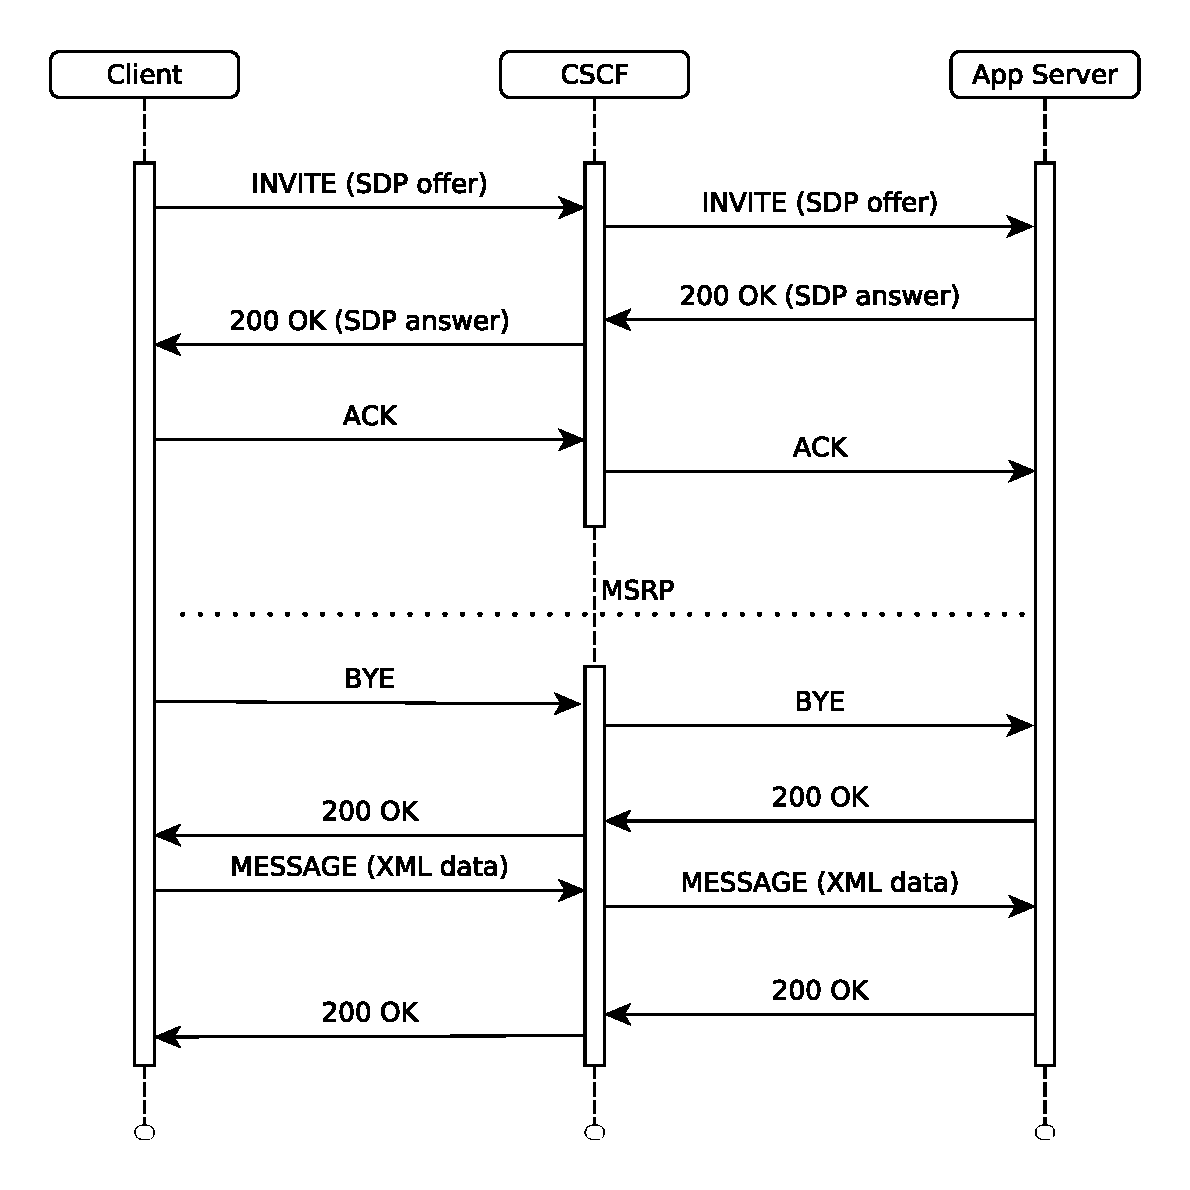
\includegraphics{img/sending_procedure.eps}}
\caption{Az üzenetküldés folyamata}
\label{fig:sending_proc}
\end{figure}

A kliens oldalon a multimédia üzenet vétele is több lépésben zajlik (\ref{fig:receiving_proc}.~ábra). Amikor a szerver új multimédia üzenetet kap, akkor a szerver első lépésként egy SIP MESSAGE üzenetben értesíti erről a címzettek közül azokat a felhasználókat, amelyek a regisztrált felhasználók listájában szerepelnek, azaz elérhetőek. Utóbbi üzenet törzse szintén XML formátumban tartalmazza a multimédia üzenetekre jellemző adatokat. Második lépésként a kliens az XML-ben kapott információk alapján eldönti, hogy kiváncsi egy adott multimédia üzenetre, vagy sem. Amennyiben érdekli maga a multimédia tartalom is, felépít egy MSRP kapcsolatot a szerver oldallal, amelyen keresztül ,,letölti'' magát a tartalmat. A felhasználó dönthet úgy, hogy jelenleg nem kiváncsi az adott multimédia üzenetre. Utóbbi esetben nincs semmilyen további kommunikáció a kliens és a szerver között. A felhasználónak lehetősége nyílik egy adott multimédia üzenet tartalom átvitele nélküli törlésére is, ilyenkor szintén SIP MESSAGE üzenetben értesíti erről a szervert. Utóbbi esetben a multimédia üzenet törlődik a felhasználó szerver oldali postafiókjából.

\begin{figure}[htbp]
\center
\resizebox{10cm}{!}{
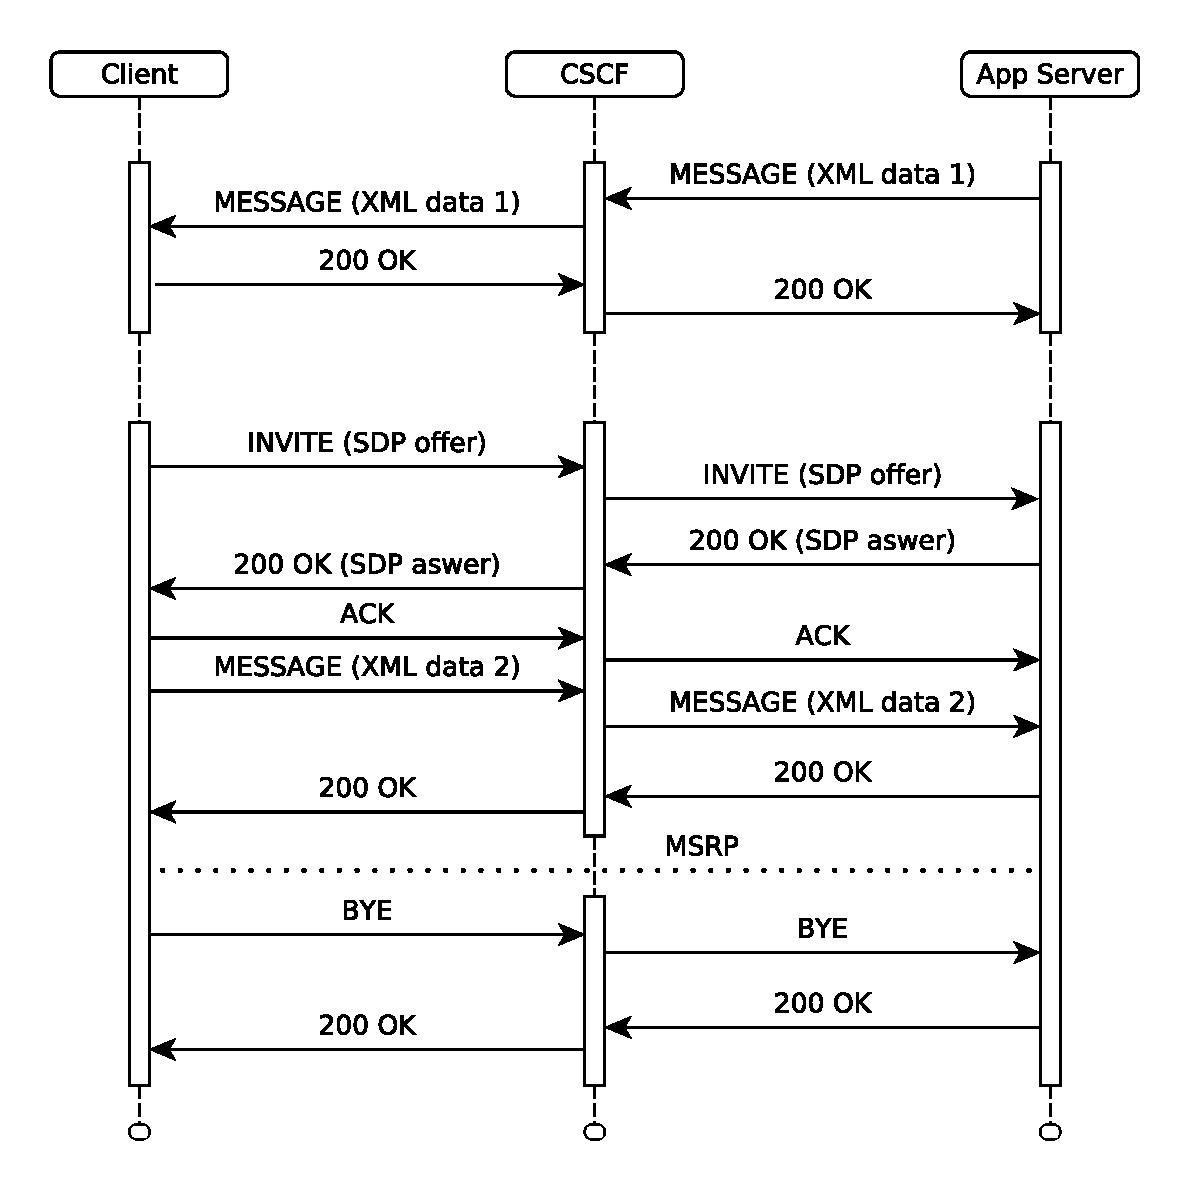
\includegraphics{img/receiving_procedure.eps}}
\caption{Az üzenet fogadás folyamata}
\label{fig:receiving_proc}
\end{figure}

\subsubsection{Alkalmazás szerver}
\label{sec:appserver}

Az alkalmazás szerver szolgáltatást nyújt a kliensek számára, az üzenetküldő rendszerben központi szerephet jut.

A szerver folyamatosan várja a kliensek csatlakozását. A szerver listát vezet a rendszerben pillanatnyilag elérhető felhasználókról. Miután a kliens oldali alkalmazás elindult, periodikusan értesíti a szervert arról, hogy elérhető a rendszerben. Egy kliens felől érkező, első regisztrációs üzenet hatására felveszi az adott klienst az elérhető kliensek listájába, majd elindít az adott felhasználóhoz egy időzítőt. Egy adott felhasználó törlése az említett listáról kétféle esemény határása történhet:
\begin{enumerate}\itemsep1pt
\item	A kliens oldali alkalmazás normális bezárásról a kliens értesíti a szervert, a\-mely\-nek hatására a szerver törli a listáról az adott felhasználót.
\item Amennyiben az időzítő lejárta előtt a szerver nem kap újabb regisztrációs üzenetet egy adott klienstől, szintén törli a felhasználót a regisztrált kliensek listájából.
\end{enumerate} 

A küldő kliens minden esetben az alkalmazás szerverrel építi fel a kapcsolatot, és annak küldi el a multimédia üzenetet. A szerver feladatai közé tartozik, hogy fogadja, majd adatbázisban eltárolja a feladótól érkező multimédia üzenetet, valamint az üzenethez kapcsolódó egyéb adatokat. Utóbbi adatok \aref{sec:kliens_pc}.~részben említett SIP MESSAGE üzenet törzsében XML formátumban érkeznek a kliens felől. Az XML a következő adatokat tartalmazza: 

\begin{itemize}\itemsep1pt
\item	A feladó SIP URI-ja
\item A címzettek SIP URI-jai
\item A üzenet azonosítója
\item Az üzenet tárgya
\item A multimédia tartalom formátuma
\end{itemize}

Az XML-ben található üzenet azonosító az MSRP átvitel során használt üzenet azonosítóval kell, hogy megegyezzek. A szerver az azonosító alapján megkeresi a kapott adatokhoz tartozó, az MSRP kapcsolaton már sikeresen átvitt, valamint adatbázisban eltárolt multimédia tartalmat, majd sikeres találat esetén hozzárendeli az XML-ből kinyert adatokat a tartalomhoz. Amennyiben a klienstől kapott azonosítóhoz nem található tartalom, hibaüzenetet küld erről a kliens oldalnak.

A szerver valósítja meg a késletetett üzenettovábbítást is. Utóbbi azt jelenti, hogy amikor a címzettek közül valamelyik nem elérhető, akkor az adott címzett értesítése az új üzenetről akkor történik meg, amikor az elérhetővé válik (azaz a kliens felől regisztrációs üzenet érkezik). Az értesítő üzenet -- hasonlóan a küldésnél használt üzenethez -- XML formátumban tartalmazza a multimédia üzenet adatait:

\begin{itemize}\itemsep1pt
\item	A feladó SIP URI-ja
\item A üzenet azonosítója
\item Az üzenet tárgya
\item A multimédia tartalom formátuma
\item A küldés dátuma
\end{itemize}

Az üzenet hatására a kliens oldal MSRP kapcsolaton a multimédia tartalom átvitelét kezdeményezheti, illetve az üzenet letöltés nélküli törlési igényét jelezheti. Az multimédia üzenet a tartalom sikeres átvitele után a szerver oldalon törlésre kerül a felhasználó fiókjából.

A kommunikáció során használt SIP MESSAGE üzenetek törzsében lévő XML tartalom szerkezetét \aref{sec:komm_uzenetek}.~fejezetben részletesen tárgyalom.

\subsubsection{Adatbázis szerver}
\label{sec:dbserver}

A küldő felhasználótól az alkalmazás szerveren keresztül érkező üzenetek átmeneti tárolását valósítja meg. Egy adott üzenethez tartozó adatok mindaddig adatbázisban tárolódnak, amíg a szerver az összes címzetthez sikeresen nem továbbította az üzenetet, vagy valamely címzettek nem jelezték az alkalmazás szerver felé, hogy ők nem kívánják megkapni az adott multimédia üzenet tényleges tartalmát. Az adatbázisban tárolásra kerülnek a feladótól érkező üzenet következő adatai:

\begin{itemize}\itemsep1pt
\item	A feladó SIP URI-ja
\item A címzettek SIP URI-jai
\item A üzenet azonosítója
\item Az üzenet tárgya
\item A multimédia tartalom
\item A multimédia tartalom formátuma
\item A küldés dátuma
\end{itemize}

\subsection{Üzemeltetési terv}
\label{sec:uzemeltetesi_terv}

Ide talán jöhetne use-case diagram, annak leírása... Vagy nem kell? Minden, ami ide jönne, már le van írva máshol is. 

\subsection{Interfész terv}
\label{sec:interfesz_terv}

Az egyes modulok közötti interfészek leírása...

Két fő komponensre különül el a rendszer fejlesztése: kliens-
ill. szerveroldali részre.

\subsubsection{Kliens}
\label{sec:kliensinterfesz}

\subsubsection{Szerver}
\label{sec:szerverinterfesz}

\subsection{Adatbázis terv}

A következő fejezetek a kommunikációs üzenetek szerkezetét, valamint a használt adatbázis felépítését tárgyalják.

\subsubsection{Kommunikációs üzenetek}
\label{sec:komm_uzenetek}

A kliens és az alkalmazás szerver közötti kommunikáció során többféle üzenettípus használatos. A kliensek regisztrációja, az MSRP kapcsolaton elküldött multimédia tartalomhoz kapcsolódó adatok átvitele, kliensek új üzenetről való értesítése SIP MESSAGE üzenetekben, XML küldésével történik. A kliens és a szerver közötti MSRP kapcsolat felépítése SIP INVITE üzenettel valósulhat meg. A multimédia tartalom átvitele MSRP csomagok formájában történik. 

\paragraph{SIP INVITE üzenetek felépítése\\}
\label{sec:sip_invite}

A kliens és a szerver közötti MSRP kapcsolat felépítése SIP és SDP protokollok használatával történik. A kapcsolatot leíró paramétereket SDP protokollal írjuk le, majd ezen adatokat SIP protokoll segítségével küldjük el a szerver oldalnak. Utóbbi azt jelenti, hogy egy SIP INVITE üzenetet küldünk a szerver oldalnak, amely üzenet törzsében az SDP-vel leírt kapcsolati információk vannak. Az alábbi üzenet bemutatja az INVITE üzenet felépítését. A kliens hasonló SIP üzenet küldésével kezdeményezi egy audió átvitelét végző MSRP kapcsolat felépítését a szerverrel.

\fontsize{10}{10}
\begin{verbatim}
INVITE sip:mediamulticast.service@ericsson.com SIP/2.0
   To: sip:server.1234@ericcson.com
   From: csaba@tmit.bme.hu
   Call-ID: 3413an89KU
   Content-Type: application/sdp

   c=IN IP4 tmit.bme.hu
   m=message 7654 TCP/MSRP *
   a=accept-types:audio/mpeg;base64
   a=path:msrp://tmit.bme.hu:7654/jshA7weztas;tcp
\end{verbatim}
\fontsize{12}{12} 

A Content-Type fejléc mező utáni üres sor az INVITE üzenet törzsének kezdetét jelzi. Látható, hogy a  törzs tartalmazza az SDP-vel leírt MSRP kapcsolat paramétereit. A példában a kliens a a tmit.bme.hu hoszton a 7654-es porton várja majd az MSRP kapcsolaton érkező csomagokat. Mivel egy adott porthoz több MSRP kapcsolat is hozzá lehet rendelve, annak érdekében, hogy az egyes kapcsolatokat meg lehessen egymástól különböztetni, a kliens generál egy egyedi kapcsolat azonosítót is. Utóbbi a path nevű argumentumban található URL elérési útjában (jshA7weztas). 

Miután a szerver oldal veszi az INVITE üzenetet, SDP protokoll alapján ő is meghatározza az MSRP kapcsolatot szerver oldalon leíró paramétereit, amelyet SIP 200 OK üzenetben továbbít a kliens felé. A fent leírt INVITE üzenetre küldött 200 OK üzenet felépítése a következő lehet:

\fontsize{10}{10}
\begin{verbatim}
SIP/2.0 200 OK
   To: sip:csaba@tmit.bme.hu
   From: sip:server.1234@ericcson.com
   Call-ID: 3413an89KU
   Content-Type: application/sdp

   c=IN IP4 ericsson.com
   m=message 7743 TCP/MSRP *
   a=accept-types:audio/mpeg;base64
   a=path:msrp://ericsson.com:7743/xyzabc45h54;tcp
\end{verbatim}
\fontsize{12}{12} 
 
Látható, hogy a szerver a 7743-as porton várja az MSRP kapcsolaton érkező csomagokat. Az MSRP kapcsolat szerver oldali azonosítója szintén a path argumentumban leírt URL-ben látható (xyzabc45h54)

A kliens oldal a 200 OK sikeres vétele után egy SIP ACK küldésével nyugtázza a szervernek a sikeres vételt. Ebben a pontban az MSRP kapcsolat sikeresen felépült a kliens és a szerver között.

\paragraph{SIP MESSAGE üzenetek felépítése\\}
\label{sec:sip_message}

A jelen dokumentumban leírt rendszerben a SIP MESSAGE típusú üzeneteket a kliensek és a szerver közötti kommunikáció során használom. Az üzenet törzsében, jól definiált XML formátumban kerülnek elküldésre a szükséges információk, mint az üzenet típusa, a feladó neve és SIP URI-ja, címzett neve és SIP URI-ja, a multimédia tartalom típusa, az üzenet tárgya, stb. Az XML tartalom az alábbi séma szerint kerül megadásra:
\fontsize{10}{10}
\begin{verbatim}
<?xml version="1.0" encoding="UTF-8"?>
<xs:schema xmlns:xs="http://www.w3.org/2001/XMLSchema"> 
<xs:element name="information">
   <xs:complexType>
      <xs:sequence>
          <!-- A üzenet típusa -->
          <xs:element name="request_type">
             <xs:simpleType>
                <xs:restriction base="xs:string">                        
                   <xs:enumeration value="STATUS_UPDATE"/>
                   <xs:enumeration value="NOTIFY"/>
                   <xs:enumeration value="DELETE_MESSAGE"/>
                   <xs:enumeration value="MESSAGE_DATA"/>
                </xs:restriction>
             </xs:simpleType>
          </xs:element>                                    
          <xs:element name="message" maxOccurs="unbounded">
             <xs:complexType>                    
                <xs:sequence>
                   <!-- STATUS_UPDATE esetén regisztráció vagy törlés -->
                   <xs:element name="status" type="xs:string" minOccurs="0"/>
                   <!-- A küldö adatai -->
                   <xs:element name="sender" minOccurs="0">
                      <xs:complexType>
                         <xs:sequence>
                            <xs:element name="name" type="xs:string"/>
                            <xs:element name="sip_uri" type="xs:string"/>
                         </xs:sequence>
                      </xs:complexType>
                   </xs:element>
                   <!-- Az üzenet azonosítója -->
                   <xs:element name="msrp_id" type="xs:string" minOccurs="0"/>
                   <!-- A multimédia tartalom típusa -->
                   <xs:element name="mime_type" type="xs:string" minOccurs="0"/>
                   <!-- Az üzenet tárgya -->
                   <xs:element name="subject" type="xs:string" minOccurs="0"/>
                   <!-- A küldés dátuma -->
                   <xs:element name="sent_at" type="xs:date" minOccurs="0"/>
                   <!-- Címzettek listája -->
                   <xs:element name="recipients" minOccurs="0">
                      <xs:complexType>
                         <xs:sequence>
                            <xs:element name="recipient" maxOccurs="unbounded">
                               <xs:complexType>
                                  <xs:sequence>
                                     <xs:element name="name" type="xs:string"/>
                                     <xs:element name="sip_uri" type="xs:string"/>
                                  </xs:sequence>
                               </xs:complexType>
                            </xs:element>
                         </xs:sequence>                    
                      </xs:complexType>                
                   </xs:element>            
                </xs:sequence>
             </xs:complexType>
          </xs:element>            
       </xs:sequence>
    </xs:complexType>
</xs:element>
</xs:schema>
\end{verbatim}
\fontsize{12}{12} 

A szóban forgó üzeneteket az alábbi esetekben használom:
\begin{mydescription}
\item[Kliens regisztráció, regisztráció törlés:] a kliens oldali alkalmazás elindulása után az al\-kal\-ma\-zás azonnal, majd periodikusan ismételve üzenetet küld a szerver oldalnak jelezvén azt, hogy a felhasználó elérhető a hálózaton. Az üzenet törzse XML formátumban tartalmazza az üzenet típusát (STATUS\_UPDATE), az üzenethez tartozó státuszt (REGISTER) valamint a felhasználó nevét és SIP URI-ját. A szerver alkalmazás a regisztrációs üzenet hatására hozzáadja a felhasználót az elérhető kliensek listájához, vagy újraindítja a listán már meglévő felhasználóhoz tartozó időzítőt. Minden felhasználóhoz tartozik egy időzítő, amely a periódusidő+$\Delta$t időtartamról számol visszafelé. A $\Delta$t egy pozitív szám, amely a változó hálózati késleltetés miatt egy biztonsági sávot nyújt az időzítőnek. Abban az esetben, ha egy periódus alatt nem érkezik egy felhasználótól ilyen regisztrációs üzenet, azaz az időzítő lejár, a szerver törli az adott felhasználót az elérhető kliensek listájából. A kliens alkalmazás bezárása esetén is ilyen típusú üzenetben értesül a szerver a kilépés eseményéről, amelynek határása szintén eltávolítja az adott klienst az elérhető felhasználókat tartalmazó listából. Utóbbi esetben az XML-ben a status mező értéke EXIT lesz.
\item[Multimédia üzenet adatainak küldése a szervernek:] az MSRP kap\-cso\-la\-ton elküldött multimédia tartalom címzetteinek adatai, illetve egyéb az üzenethez kapcsolódó információk átvitele is ilyen típusú üzenetben történik. Ebben az esetben a kliens oldal a SIP MESSAGE üzenetet azután küldi el a szerver oldalnak, miután a multimédia üzenethez kapcsolódó tartalom az MSRP kapcsolaton sikeresen továbbítódott.
\item[Új üzenetről értesítés:] amikor egy felhasználó új multimédia üzenetet kap, a szerver a szóban forgó üzenetben értesíti az új üzenetről, vagy több üzenet esetén az új üzenetekről a kliens oldalt. Az üzenet tartalmazza a feladó adatait, illetve az üzenetek adatait (mint például az üzenet azonosítóját, a tartalom típusát, az üzenet tárgyát, stb.).
\item[Üzenet törlési igényének küldése a szerver felé:] a szerver sikeresen értesítette a felhasználót az új multimédia üzenetről, de a felhasználó úgy dönt, hogy megtekintés nélkül törölni kívánja a szóban forgó multimédia üzenet tartalmát, akkor efy SIP MESSAGE üzenetben értesíti erről a szervert. A SIP kérés típusa ebben az esetben DELETE\_MESSAGE, amely tartalmazni fogja a törölni kívánt multimédia üzenet azonosítóját is.

\end{mydescription}

\paragraph{MSRP csomagok felépítése\\}
\label{sec:msrp_chunks}

A multimédia tartalom MSRP kapcsolaton kerül átvitelre, amely kapcsolaton MSRP csomagok formájában történik a kommunikáció. Egy MSRP üzenetváltás két lépésből áll. A küldő fél egy msrp kérést küld a fogadó félnek, amit a fogadó fél nyugtázik. A kérés küldés -- fogadás -- nyugtázás lépések együttesét tranzakciónak nevezik. Tehát fő MSRP üzenettípus létezik:
\begin{myenumerate}
\item \label{enum:msrp_req} MSRP kérés
\item \label{enum:msrp_resp} MSRP válasz
\end{myenumerate}
\bigskip

\noindent
{\bf \ref{enum:msrp_req}.~MSRP kérés}

Az msrp kérés struktúrális felépítése rendszerint három részből áll: fejléc, törzs, valamint egy záró sor. A fejléc tartalmazza többek között az üzenet azonosítóját, a tranzakció azonosítót, az MSRP kapcsolat azonosítóját, illetve a forrást és a célt leíró URI-kat. Amennyiben a kérés törzsében tartalom kerül átvitelre, abban az esetben a tartalmat leíró információk is megtalálhatóak a fejlécben (a tartalom típusa, hossza). A záró sor szabvány szerint hét darab ,,-'' jelből, a tranzakció azonosítóból és a ,,\$'', ,,+'' vagy ,,\#'' karakterek egyikéből épül fel. Mivel egy üzenet darabolva, több msrp kérésben kerülhet átvitelre, a záró sor utolsó karaktere attól függ, hogy az adott kérés ugyanazon üzenet egy köztes részét tartalmazza (+~jel), az üzenet utolsó darabját tartalmazza (\$~jel), vagy az üzenet küldését megszakították (\#~jel). Az alábbi két msrp kérés az ,,abcdefGHIJKL'' üzenet két darabban történő átvitelét szemlélteti:

\fontsize{10}{10}
\begin{verbatim}
MSRP 1a2b3c4d SEND
To-Path: msrp://syrius.bme.hu:12763/kjhd37s2s20w2a;tcp
From-Path: msrp://csb.invitel.hu:7654/jshA7weztas;tcp
Message-ID: abcd9876
Byte-Range: 1-6/12
Content-Type: text/plain

abcdef
-------1a2b3c4d+

MSRP 5e6f7g8h SEND
To-Path: msrp://syrius.bme.hu:12763/kjhd37s2s20w2a;tcp
From-Path: msrp://csb.invitel.hu:7654/jshA7weztas;tcp
Message-ID: abcd9876
Byte-Range: 7-12/12
Content-Type: text/plain

GHIJKL
-------5e6f7g8h$
\end{verbatim}
\fontsize{12}{12} 

A csoportos multimédia üzenetküldő rendszerben a multimédia tartalom átvitele msrp kérésekben, base64 kódolva\footnote{RFC4648: The Base16, Base32, and Base64 Data Encodings \cite{rfc4648}} kerül átvitelre. A kódolás célja, hogy a bináris, speciális karaktereket tartalmazó adatokból ASCII\footnote{American Standard Code for Information Interchange} karaktersorozatot állít elő, ezáltal a vételi oldalon az eredeti multimédia tartalom egy base64 dekódolással egyértelműen visszaállítható lesz.
\bigskip

\noindent
{\bf \ref{enum:msrp_resp}.~MSRP válasz}

Az msrp válasz felépítése megegyezik az msrp kérés felépítésével, azzal a különbséggel, hogy az msrp válaszban nincs tartalom átvitel, ezáltal a törzs rész hiányzik. Az előző részben illusztrált két msrp kérésre sikeres kézbesítés esetén az alábbi msrp válaszok jönnek:
\fontsize{10}{10}
\begin{verbatim}
MSRP 1a2b3c4d 200 OK
To-Path: msrp://csb.invitel.hu:7654/jshA7weztas;tcp
From-Path: msrp://syrius.bme.hu:12763/kjhd37s2s20w2a;tcp
-------1a2b3c4d$

MSRP 5e6f7g8h 200 OK
To-Path: msrp://csb.invitel.hu:7654/jshA7weztas;tcp
From-Path: msrp://syrius.bme.hu:12763/kjhd37s2s20w2a;tcp
-------5e6f7g8h$
\end{verbatim}
\fontsize{12}{12} 

\bigskip

Az MSRP protokollról, a csomagok felépítéséről részletesebben a \cite{rfc4975} és a \cite{rfc4976} irodalomban olvashat.

\subsubsection{Az adatbázis}
\label{sec:adatb}

A multimédia üzenet tárolásához egy relációs adatbázisra van szükség. Mivel a Java nyelvben az SQL alapú relációs adatbázisok használatára már kiforrott API áll rendelkezésre, az SQL alapú relációs adatbázis-kezelő szerverek közül célszerű választani. A fejlesztés során a MySQL adatbázis-kezelő szerverre esett a választás, mivel széles közben elérhető, illetve Java nyelvre megtalálható hozzá egyedi illesztőfelület.

Az adatbázis felépítéséhez az alábbi táblákra lesz szükség:

\begin{myitemize}
\item A multimédia üzenet tárolásához,
\item a multimédia üzenet címzettjeinek tárolásához
\end{myitemize}

A következőkben ezen pontok részletezésére kerül sor.

\paragraph*{A multimédia üzenet tárolása\\}

Az alábbi szerkezetű tábla szükséges az egyes multimédia üzenethez kapcsolódó adatok tárolásához:
\fontsize{10}{10}
\begin{verbatim}
CREATE TABLE MESSAGES
(
  ID INT NOT NULL AUTO_INCREMENT,
  MSRP_MESSAGE_ID VARCHAR(200) NOT NULL,
  CONTENT BLOB
  SENDER_NAME VARCHAR(150)
  SENDER_SIP_URI VARCHAR(150)
  SENT_AT DATE
  SUBJECT VARCHAR(250)
  CONTENT_TYPE VARCHAR(50),
  CONSTRAINT pk_messages PRIMARY KEY(ID),
  CONSTRAINT uq_msrp_message_id UNIQUE(MSRP_MESSAGE_ID)
) ENGINE=InnoDB DEFAULT CHARSET=utf8;
\end{verbatim}
\fontsize{12}{12}

Az egyes adatmezők jelentése:
\begin{mydescription}
\item[ID:] a tábla sorainak egyértelmű azonosítására szolgál, a tábla elsődleges kulcsa. Értelemszerűen nem vehet fel NULL értéket.
\item[MSRP\_MESSAGE\_ID:] az MSRP kapcsolaton átvitt multimédia tartalom MSRP azonosítója, amely egy véletlen karakterlánc. A mező alapján egyértelműen visszakereshető a multimédia üzenet. Értéke egyedi a táblában, továbbá nem vehet fel NULL értéket. A multimédia tartalom MSRP kapcsolaton történő sikeres átvitele után ezen azonosító alapján küldi el az üzenethez kapcsolódó további adatokat, mint a címzettek, az üzenet tárgya, a tartalom formátuma, stb. (lásd. \ref{sec:appserver}.~ fejezet) 
\item[CONTENT:] ebben a mezőben a multimédia üzenethez tartozó multimédia tartalom base64 kódolt bájtfolyamként tárolódik.
\item[SENDER\_NAME:] az üzenet feladójának nevét tartalmazó oszlop.
\item[SENDER\_SIP\_URI:] az üzenetet feladó felhasználó SIP URI-jának tárolására szolgáló mező.
\item[SENT\_AT:] az üzenet küldésének a dátuma. 
\item[SUBJECT:] a multimédia üzenethez tartozó rövid szöveges tárgymező.
\item[CONTENT\_TYPE:] a multimédia tartalom MIME típusa. (típus/altípus formában eltárolva. például: video/mpeg)
\end{mydescription}
\medskip

\paragraph*{A multimédia üzenet címzettjeinek tárolása\\}

A címzettek tárolásához a következő szerkezetű tábla szükséges:
\fontsize{10}{10}
\begin{verbatim}
CREATE TABLE RECIPIENTS
(
  ID INT NOT NULL AUTO_INCREMENT,
  MESSAGE_ID INT NOT NULL,
  NAME VARCHAR(150)
  SIP_URI VARCHAR(150)
  DELIVERY_STATUS VARCHAR(30)
  CONSTRAINT pk_recipients PRIMARY KEY (ID)
  CONSTRAINT fk_messages FOREIGN KEY (MESSAGE_ID) REFERENCES MESSAGES(ID)
) ENGINE=InnoDB DEFAULT CHARSET=utf8;
\end{verbatim}
\fontsize{12}{12}

Az egyes adatmezők jelentése:
\begin{mydescription}
\item[ID:] a tábla elsődleges kulcsa, a tábla sorainak egyértelmű azonosítására szolgál. Értéke szekvenciálisan növekszik. Elsődleges kulcs révén természetesen nem vehet fel NULL értéket.
\item[MESSAGE\_ID:] idegen kulcs a címzetthez rendelt multimédia üzenet rekordjára. A mező alapján rendeljük hozzá a címzettet egy adott multimédia üzenethez.
\item[NAME:]  a címzett nevét tartalmazó oszlop.
\item[SIP\_URI:] a címzett SIP azonosítóját tartalmazó mező.
\item[DELIVERY\_STATUS:] az adott címzetthez rendelt multimédia üzenet kézbesítési állapotát írja le. Értéke új és még kézbesítetlen üzenet esetén NEW. Abban az esetben, ha az alkalmazás szerver sikeresen értesítette a címzettet az új multimédia üzenetről, a státusz értéke NOTIFIED értéket kap. Ha a címzett ezek után kezdeményezte, majd MSRP kapcsolaton keresztül sikeresen letöltötte a multimédia üzenetet, értéke SENT állapotba kerül. Végül, ha a címzett előzetes átvitel nélkül jelezte a szerver felé, hogy nem kívánja letölteni az üzenetet, amely így törölhető, a mező DELETED értéket kap.
\end{mydescription}

\medskip

\subsection{Megvalósítási terv}
\label{sec:megvalositas}

Ide jönnek majd az állapotgépek, működés leírása...

\subsubsection{A kliens megvalósítása}
\label{sec:kliensmegvalositas}

\subsubsection{A szerver megvalósítása}
\label{sec:szervermegvalositas}


\subsection{Összefoglalás}

